\documentclass[tikz,border=7pt]{standalone}
% Shared TikZ style for the Nios V stereo accelerator diagrams.
\usepackage[T1]{fontenc}
\usepackage{lmodern}
\usepackage{xcolor}
\usepackage{tikz}
\usetikzlibrary{arrows.meta,backgrounds,calc,fit,positioning}

\definecolor{navy}{HTML}{073D73}
\definecolor{blue}{HTML}{0B5CAB}
\definecolor{cyan}{HTML}{1B8DBB}
\definecolor{green}{HTML}{27845B}
\definecolor{orange}{HTML}{C66A16}
\definecolor{red}{HTML}{B94444}
\definecolor{ink}{HTML}{172033}
\definecolor{muted}{HTML}{5A6678}
\definecolor{line}{HTML}{BFCBDA}
\definecolor{softblue}{HTML}{EDF4FA}
\definecolor{softcyan}{HTML}{ECF8FB}
\definecolor{softgreen}{HTML}{EEF8F2}
\definecolor{softorange}{HTML}{FFF4E8}
\definecolor{softgray}{HTML}{F5F7FA}

% Avoid automatic word hyphenation inside compact diagram nodes.
\hyphenpenalty=10000
\exhyphenpenalty=10000

\tikzset{
  font=\sffamily,
  block/.style={
    draw=line, rounded corners=2.2pt, fill=white,
    minimum height=10mm, text width=31mm, align=center,
    inner xsep=3mm, inner ysep=2.2mm
  },
  cpu/.style={block, draw=blue!55, fill=softblue},
  accel/.style={block, draw=cyan!65, fill=softcyan},
  memory/.style={block, draw=green!60, fill=softgreen},
  control/.style={block, draw=orange!65, fill=softorange},
  smallblock/.style={block, text width=24mm, minimum height=8mm, inner xsep=2mm, inner ysep=1.6mm},
  group/.style={draw=line, rounded corners=4pt, fill=softgray, inner sep=4mm},
  labeltag/.style={rounded corners=2pt, fill=navy, text=white, font=\sffamily\bfseries\footnotesize, inner xsep=2.5mm, inner ysep=1.2mm},
  flow/.style={-{Stealth[length=2.6mm,width=1.8mm]}, draw=navy, line width=0.85pt},
  dataflow/.style={-{Stealth[length=2.8mm,width=2mm]}, draw=blue, line width=1.15pt},
  controlflow/.style={-{Stealth[length=2.4mm,width=1.7mm]}, draw=orange, line width=0.9pt, dashed},
  returnflow/.style={-{Stealth[length=2.4mm,width=1.7mm]}, draw=green, line width=0.9pt},
  bus/.style={<->, >={Stealth[length=2.8mm,width=2mm]}, draw=navy, line width=1.6pt},
  note/.style={font=\sffamily\footnotesize, text=muted, align=left},
  arrowlabel/.style={font=\sffamily\scriptsize, text=muted, fill=white, inner sep=1.2pt}
}


\begin{document}
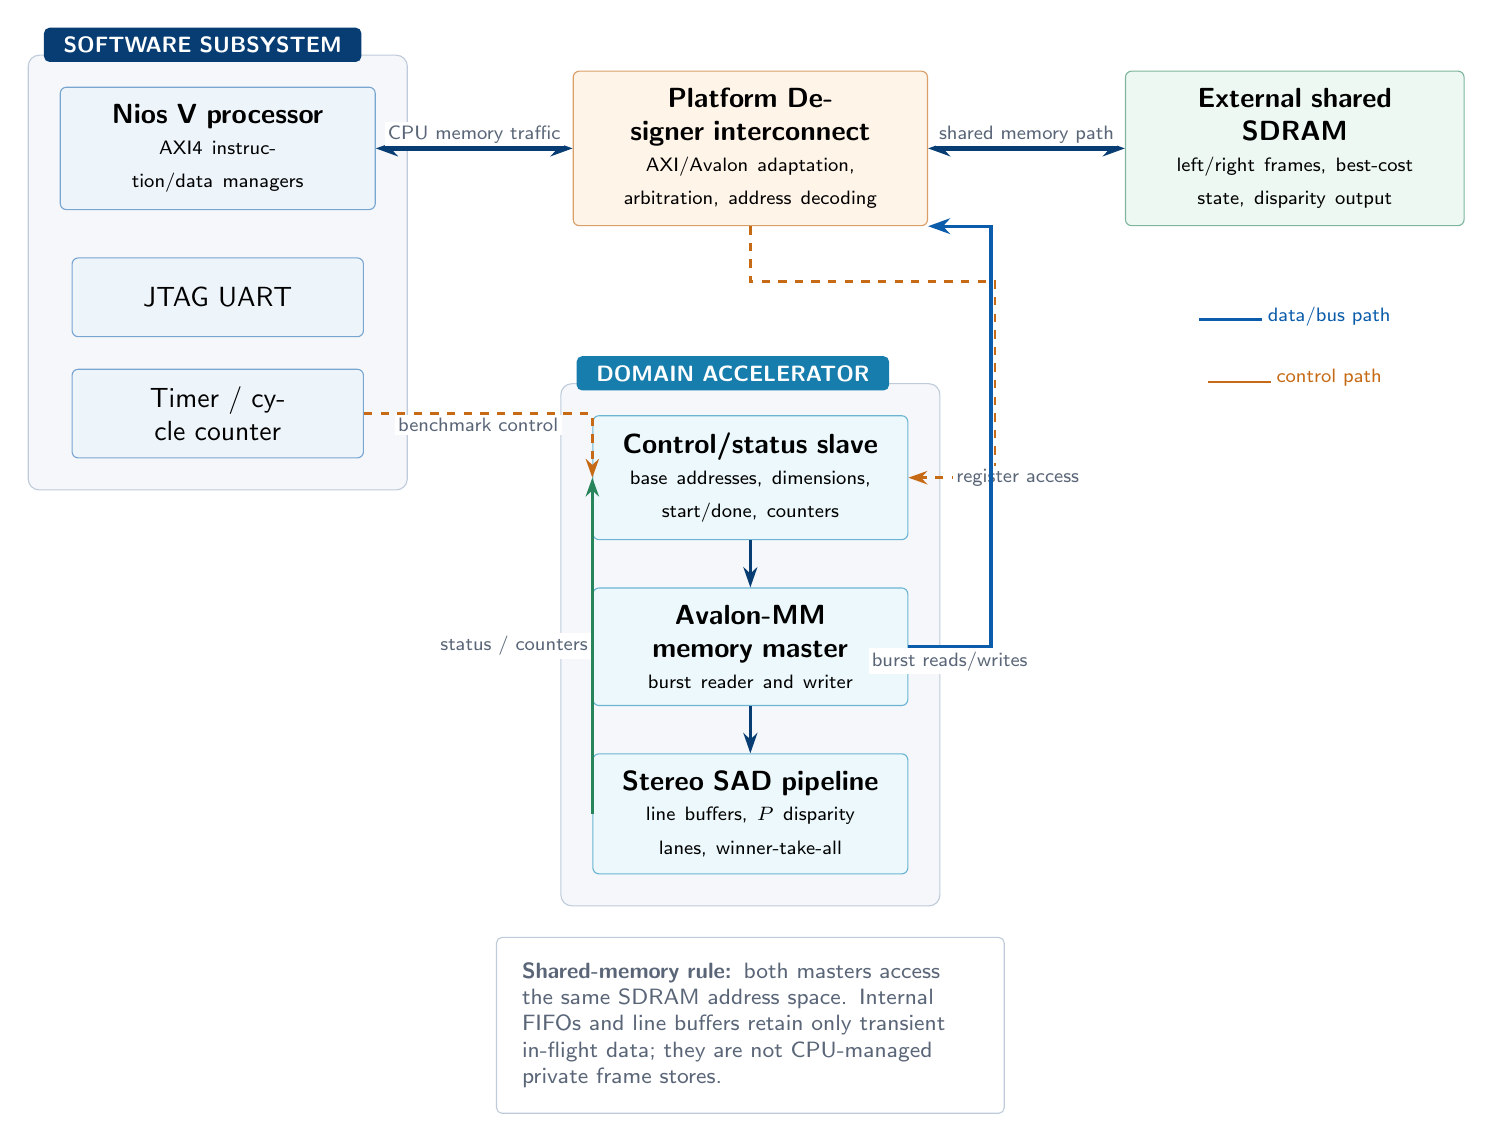
\begin{tikzpicture}[node distance=11mm and 15mm]
  % CPU subsystem
  \node[cpu, text width=34mm] (cpu) {\textbf{Nios V processor}\\[-1pt]\scriptsize AXI4 instruction/data managers};
  \node[smallblock, cpu, below=6mm of cpu] (jtag) {JTAG UART};
  \node[smallblock, cpu, below=4mm of jtag] (timer) {Timer / cycle counter};
  \begin{scope}[on background layer]
    \node[group, fit=(cpu)(jtag)(timer)] (cpugroup) {};
  \end{scope}
  \node[labeltag, anchor=south west] at ([xshift=2mm,yshift=-1mm]cpugroup.north west) {SOFTWARE SUBSYSTEM};

  % Interconnect
  \node[control, text width=39mm, right=25mm of cpu] (fabric) {\textbf{Platform Designer interconnect}\\[-1pt]\scriptsize AXI/Avalon adaptation, arbitration, address decoding};

  % SDRAM
  \node[memory, text width=37mm, right=25mm of fabric] (sdram) {\textbf{External shared SDRAM}\\[-1pt]\scriptsize left/right frames, best-cost state, disparity output};

  % Accelerator subsystem
  \node[accel, text width=34mm, below=24mm of fabric] (ctrl) {\textbf{Control/status slave}\\[-1pt]\scriptsize base addresses, dimensions, start/done, counters};
  \node[accel, text width=34mm, below=6mm of ctrl] (master) {\textbf{Avalon-MM memory master}\\[-1pt]\scriptsize burst reader and writer};
  \node[accel, text width=34mm, below=6mm of master] (pipeline) {\textbf{Stereo SAD pipeline}\\[-1pt]\scriptsize line buffers, $P$ disparity lanes, winner-take-all};
  \begin{scope}[on background layer]
    \node[group, fit=(ctrl)(master)(pipeline)] (accgroup) {};
  \end{scope}
  \node[labeltag, anchor=south west, fill=cyan!80!navy] at ([xshift=2mm,yshift=-1mm]accgroup.north west) {DOMAIN ACCELERATOR};

  % Connections
  \draw[bus] (cpu.east) -- node[arrowlabel, above] {CPU memory traffic} (fabric.west);
  \draw[bus] (fabric.east) -- node[arrowlabel, above] {shared memory path} (sdram.west);
  \draw[controlflow] (fabric.south) -- ++(0,-7mm) -| ([xshift=11mm]ctrl.east) |- node[arrowlabel, near end, right] {register access} (ctrl.east);
  \draw[dataflow] (master.east) -| node[arrowlabel, near start, below] {burst reads/writes} ([xshift=8mm]fabric.south east) |- (fabric.south east);
  \draw[flow] (ctrl.south) -- (master.north);
  \draw[flow] (master.south) -- (pipeline.north);
  \draw[returnflow] (pipeline.west) -| node[arrowlabel, near end, left] {status / counters} (ctrl.west);
  \draw[controlflow] (timer.east) -| node[arrowlabel, near start, below] {benchmark control} (ctrl.west);

  % Shared-memory requirement annotation
  \node[note, text width=58mm, below=10mm of pipeline] (note) {\textbf{Shared-memory rule:} both masters access the same SDRAM address space. Internal FIFOs and line buffers retain only transient in-flight data; they are not CPU-managed private frame stores.};
  \draw[draw=line, rounded corners=2pt] ([xshift=-2mm,yshift=-2mm]note.south west) rectangle ([xshift=2mm,yshift=2mm]note.north east);

  % Legend
  \node[font=\sffamily\scriptsize, text=blue, below=9mm of sdram] (ld) {\rule{8mm}{1.1pt}\;data/bus path};
  \node[font=\sffamily\scriptsize, text=orange, below=3mm of ld] {\rule{8mm}{0.7pt}\;control path};
\end{tikzpicture}
\end{document}
